%!TEX TS-program = xelatex
\documentclass[a4paper,14pt]{article}

% В этом документе преамбула

%%% Работа с русским языком
\usepackage{cmap}					% поиск в PDF
\usepackage{mathtext} 				% русские буквы в формулах
%\usepackage[T2A]{fontenc}			% кодировка
%\usepackage[utf8]{inputenc}			% кодировка исходного текста
\usepackage[english,russian]{babel}	% локализация и переносы
\usepackage{indentfirst}
\frenchspacing

%%%Шрифты
\usepackage{fontspec}      %% подготавливает загрузку шрифтов Open Type, True Type и др.
\defaultfontfeatures{Ligatures={TeX},Renderer=Basic}  %% свойства шрифтов по умолчанию
\setmainfont[Ligatures={TeX,Historic}]{Times New Roman} %% задаёт основной шрифт документа
\setsansfont{Carlito}                    %% задаёт шрифт без засечек
\setmonofont{Courier New}

\renewcommand{\epsilon}{\ensuremath{\varepsilon}}
\renewcommand{\phi}{\ensuremath{\varphi}}
\renewcommand{\kappa}{\ensuremath{\varkappa}}
\renewcommand{\le}{\ensuremath{\leqslant}}
\renewcommand{\leq}{\ensuremath{\leqslant}}
\renewcommand{\ge}{\ensuremath{\geqslant}}
\renewcommand{\geq}{\ensuremath{\geqslant}}
\renewcommand{\emptyset}{\varnothing}

%%% Дополнительная работа с математикой
\usepackage{amsmath,amsfonts,amssymb,amsthm,mathtools} % AMS
\usepackage{icomma} % "Умная" запятая: $0,2$ --- число, $0, 2$ --- перечисление

%% Номера формул
%\mathtoolsset{showonlyrefs=true} % Показывать номера только у тех формул, на которые есть \eqref{} в тексте.
%\usepackage{leqno} % Нумереация формул слева

%% Свои команды
\DeclareMathOperator{\sgn}{\mathop{sgn}}

%% Перенос знаков в формулах (по Львовскому)
\newcommand*{\hm}[1]{#1\nobreak\discretionary{}
{\hbox{$\mathsurround=0pt #1$}}{}}

%%% Работа с картинками
\usepackage{graphicx}  % Для вставки рисунков
\graphicspath{{images/}{images2/}}  % папки с картинками
\setlength\fboxsep{3pt} % Отступ рамки \fbox{} от рисунка
\setlength\fboxrule{1pt} % Толщина линий рамки \fbox{}
\usepackage{wrapfig} % Обтекание рисунков текстом

%%% Работа с таблицами
\usepackage{array,tabularx,tabulary,booktabs} % Дополнительная работа с таблицами
\usepackage{longtable}  % Длинные таблицы
\usepackage{multirow} % Слияние строк в таблице

%%% Теоремы
\theoremstyle{plain} % Это стиль по умолчанию, его можно не переопределять.
\newtheorem{theorem}{Теорема}[section]
\newtheorem{proposition}[theorem]{Утверждение}
 
\theoremstyle{definition} % "Определение"
\newtheorem{corollary}{Следствие}[theorem]
\newtheorem{problem}{Задача}[section]
 
\theoremstyle{remark} % "Примечание"
\newtheorem*{nonum}{Решение}

%%% Программирование
\usepackage{etoolbox} % логические операторы

%%% Страница
\usepackage{extsizes} % Возможность сделать 14-й шрифт
\usepackage{geometry} % Простой способ задавать поля
	\geometry{top=25mm}
	\geometry{bottom=35mm}
	\geometry{left=35mm}
	\geometry{right=20mm}
 %
%\usepackage{fancyhdr} % Колонтитулы
% 	\pagestyle{fancy}
 	%\renewcommand{\headrulewidth}{0pt}  % Толщина линейки, отчеркивающей верхний колонтитул
% 	\lfoot{Нижний левый}
% 	\rfoot{Нижний правый}
% 	\rhead{Верхний правый}
% 	\chead{Верхний в центре}
% 	\lhead{Верхний левый}
%	\cfoot{Нижний в центре} % По умолчанию здесь номер страницы

\usepackage{setspace} % Интерлиньяж
\onehalfspacing % Интерлиньяж 1.5
%\doublespacing % Интерлиньяж 2
%\singlespacing % Интерлиньяж 1

\usepackage{lastpage} % Узнать, сколько всего страниц в документе.

\usepackage{soul} % Модификаторы начертания

\usepackage{hyperref}
\usepackage[usenames,dvipsnames,svgnames,table,rgb]{xcolor}
\hypersetup{				% Гиперссылки
    unicode=true,           % русские буквы в раздела PDF
    pdftitle={NIR2},   % Заголовок
    pdfauthor={Dmitry Velikiy},      % Автор
    pdfsubject={master's nir №2},      % Тема
    pdfcreator={Dmitry Velikiy}, % Создатель
    pdfproducer={Dmitry V.}, % Производитель
    pdfkeywords={modelling} {forecast} {social}, % Ключевые слова
    colorlinks=false,       	% false: ссылки в рамках; true: цветные ссылки
    linkcolor=red,          % внутренние ссылки
    citecolor=black,        % на библиографию
    filecolor=magenta,      % на файлы
    urlcolor=cyan           % на URL
}

\usepackage{csquotes} % Еще инструменты для ссылок

%Библиография
\usepackage[backend=biber,bibencoding=utf8,sorting=nty,maxcitenames=4,style=gost-numeric, language=auto, babel=other]{biblatex}
\addbibresource{fuzzy_thesis.bib}

\usepackage{multicol} % Несколько колонок

\usepackage{tikz} % Работа с графикой
\usepackage{pgfplots}
\usepackage{pgfplotstable}
\usepackage{pgfcalendar}

%Счетчик страниц
\usepackage{lastpage}

\author{Дмитрий Великий}
\title{НИР №1}
\date{\today}

\begin{document} % конец преамбулы, начало документа


\tableofcontents

\newpage
\section*{\centering Реферат}
\addcontentsline{toc}{section}{Реферат}
Отчет \pageref{LastPage} с., 3 ч., 2 рис., 15 источников.

\textbf{Тема:} Нечеткое прогнозирование временных рядов.

\textbf{Объектом исследования} являются методы прогнозирования временных рядов.

\textbf{Предмет исследования:} применимость различных методов прогнозирования к задачам регионального управления.

\textbf{Цель работы:} анализ применимости новых моделей прогнозирования к задачам государственного управления.

\textbf{Поставленные задачи} для достижения цели НИР:
\begin{itemize}
	\item обзор литературы по теме прогнозирования временных рядов, и в особенности, интеллектуального прогнозирования.
	\item выявление сфер применения новых методов прогнозирования, степени их теоретической проработки и практических результатов их использования.
	\item обзор программных пакетов, позволяющих реализовывать методы нечеткого прогнозирования.
\end{itemize}

\newpage
\section*{Введение}
\addcontentsline{toc}{section}{Введение}

Цель данной работы – анализ применимости новых моделей прогнозирования к задачам государственного управления.

Для достижения указанной цели необходимо решить следующие задачи:
\begin{enumerate}
    \item обзор литературы по теме прогнозирования временных рядов, и в особенности, интеллектуального прогнозирования
    \item выявление сфер применения новых методов прогнозирования, степени их теоретической проработки и практических результатов их использования.    
    \item обзор программных пакетов, позволяющих реализовывать методы нечеткого прогнозирования.
\end{enumerate}
Работа выполняется по заказу Санкт-Петербургского информационно-аналитического центра.

\newpage
\section{Задачи прогнозирования и интеллектуальный анализ временных рядов}

Количество информации, порождаемой человечеством, непрерывно растет \cite{Gantz2011}. 
В связи с этим все важнее становится умение анализировать данные, извлекать из них знания, чтобы превратить в движущую силу социально-экономического развития. 

Одним из методов анализа данных является прогнозирование. 
Прогнозная аналитика использует методы математического моделирования, искусственного интеллекта и теории игр, 
анализирует текущие и исторические факты для составления предсказаний о будущих событиях. 
Фиксируются связи между разными факторами, на основании их выявления идентифицируются риски и возможности. 
Задача прогнозирования лежит в основе финансового планирования в экономике, управления объемами производства, принятия решений в сфере управления социальными системами.

На сегодняшний день существует множество моделей прогнозирования временных рядов \cite{Chuchueva2012}: регрессионные и авторегрессионные, 
нейросетевые, экспоненциального сглаживания, на базе цепей Маркова, классификационные и др. (Рис. ~\ref{figure:mod_classifier}).
\begin{figure}[bhtp]
    \centering
    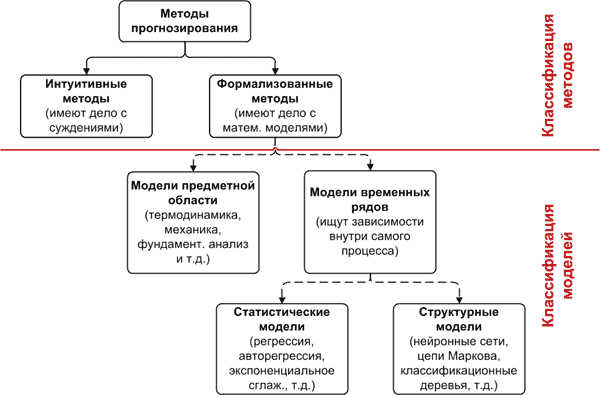
\includegraphics[width=\textwidth, keepaspectratio]{images/mod_classifier.png}
    \caption{классификация моделей и методов прогнозирования \cite{Chuchueva13habr}}
    \label{figure:mod_classifier}
\end{figure}
Прогнозирование в государственном управлении осуществляется посредством разных методов: экстраполяции, факторного прогнозирования, 
модельного прогнозирования, экспертного оценивания. 
Органы государственной власти в последние годы все чаще обращаются к методу экспертного прогнозирования \cite{Gegedush2008}. 
В этом случае эксперт дает прогноз, опираясь на опыт, аналогии, интуицию. 
В то же время интуитивная природа данного метода заставляет при его использовании полагаться лишь на квалификацию и репутацию эксперта, 
тем самым внося дополнительную неопределенность в процесс прогнозирования. 
Существуют исследования, показывающие, что прогнозы экспертов по точности уступают прогнозам на основе моделирования. 
П. Мийл на примере 20 прогнозов из области клинической диагностики \cite{MeehlClinStat} 
и Дж. Сойер на примере 45 прогнозов в социальной сфере \cite{Sawyer1966} демонстрируют тот факт, 
что экспертные оценки ни в одном из перечисленных случаев не были существенно точнее статистических моделей прогнозирования. 
Кроме того, наблюдается нехватка специалистов по работе с данными \cite{Davenport2012}. 
Все это побуждает задуматься о других подходах к анализу данных. 

В последние два десятилетия активно развивается направление прогнозирования, связанное с интеллектуальным анализом временных рядов \cite{Yarushkina2010}. 
Основными целями этого направления являются, во-первых, анализ и моделирование процессов, характеризующихся высокой степенью неопределенности, 
в том числе в областях, слабо подверженных формализации, 
во-вторых, повышение уровня интеллектуальной поддержки современных специалистов, 
и, в-третьих, выявление скрытых закономерностей и извлечение новых знаний из временных рядов. 

\newpage
\section{Сферы применения методов интеллектуального анализа временных рядов}

В основе новых методов анализа временных рядов лежит нечеткая модель временного ряда. 
Теория нечетких множеств была впервые изложена Л. Заде в 1965 г. \cite{zadeh1965fuzzy}. 
В 1973 г. предложена теория нечеткой логики \cite{Zadeh1973}. 
Вскоре после этого теория стала популярна. 
В конце 1980-х гг. это направление стало бурно развиваться в Японии. 
Нечеткое управление стало применяться в промышленности, железнодорожном транспорте и разработке потребительской техники.

\begin{figure}[h]
    \centering
    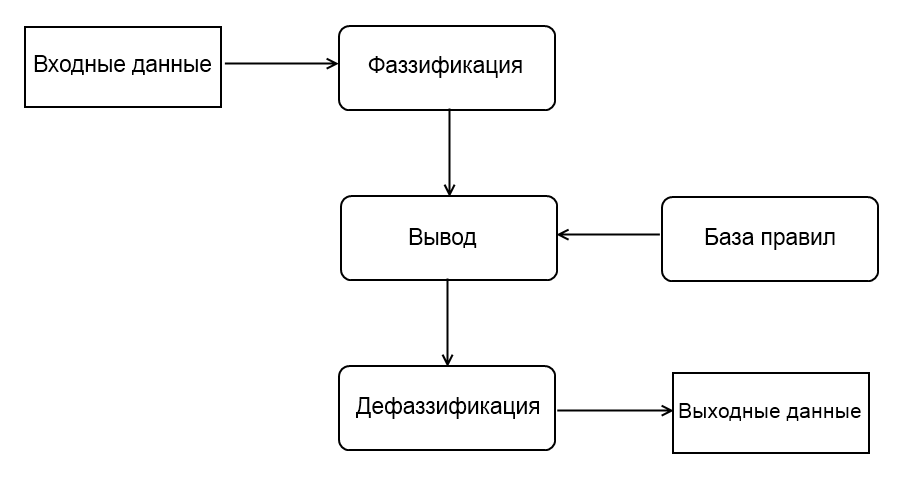
\includegraphics[width=\textwidth, keepaspectratio]{images/fuzzy_engine.png}
    \caption{Система нечеткого вывода}
    \label{figure:fuzzy_engine}
\end{figure}

Основной идеей нечеткой логики является многозначность. 
Высказывание может иметь любое истинностное значение в промежутке от 0 до 1. 
Таким образом, воспроизводится неточность человеческого мышления.

Модели статических и динамических систем, построение, 
использование и анализ которых базируется на положениях теории нечетких множеств и нечеткой логики, называют нечеткими моделями или нечеткими системами. 
Целью нечеткого моделирования сложных явлений является приближенное описание зависимости. 

В основе нечетких продукционных моделей лежит совокупность нечетких правил «ЕСЛИ, ТО», 
описывающих зависимости между нечеткими переменными предметной области, 
композиционное правило вывода и способ вычисления значений нечетких переменных (способ нечеткого вывода).

Модель описания поведения систем на естественном (или близком к естественному) языке,
в виде приближенных рассуждений в теории нечетких множеств и нечеткой логики,
основанная на композиционном правиле вывода, называется системой нечеткого логического вывода.

В систему нечеткого логического вывода входят следующие объекты (рис. ~\ref{figure:fuzzy_engine}):
\begin{enumerate} 
    \item совокупность нечетких продукционных правил (база правил);
    \item блок фаззификации;
    \item блок дефаззификации;
    \item блок вывода.
\end{enumerate}

На основании общей модели, приведенной выше, создаются контроллеры для управления преимущественно техническими объектами.

В начале 1990-х гг. была предложена теория нечетких временных рядов \cite{Song1993}. 
Нечетким временным рядом называют упорядоченную в равноотстоящие моменты времени последовательность наблюдений над некоторым процессом,
состояния которого изменяются во времени, если значение состояния процесса в данный момент времени может быть выражено с помощью нечеткой метки. 
Нечеткая метка может быть сформирована непосредственно экспертом или получена на основе некоторого преобразования исходного временного ряда \cite{Yarushkina2010}. 

В условиях, когда моделируемым процессам присуща высокая степень неопределенности, 
методы прогнозирования на основе нечетких моделей временных рядов позволяют выработать наиболее адекватную оценку будущих изменений в социально-экономических системах.

Ряд исследований \cite{Chen1996,S.Melike2008,Saxena2012}, в которых изучается прогнозирование с помощью моделей нечетких временный рядов, 
демонстрирует положительные результаты. 
Точность прогнозирования улучшается за счет использования генетических алгоритмов для настройки параметров нечетких моделей прогнозирования, 
изменения количества нечетких множеств, используемых для описания временного ряда, использование достаточного числа продукционных правил, 
модификации интервалов, на которые разбивается исходный ряд и др.

В то же время есть примеры неудовлетворительного применения нечеткой логики в прогнозировании временных рядов \cite{Hoekstr2010}. 
Причиной тому неопределенность при создании набора продукционных правил, необходимость адекватного выбора переменных, 
включаемых в модель, сложность построения модели ввиду новизны, малой изученности данной темы и большой вариативности при построении модели.

\newpage
\section{Программные средства интеллектуального прогнозирования}

Для использования прогнозирования в принятии решений целесообразным может оказаться интеграция этих моделей с экспертной системой или системой поддержки принятия решений. 
В этом случае нужно задуматься о программной реализации нечетко-логических моделей. 
Попробуем рассмотреть существующие библиотеки, в той или иной мере охватывающие тему нечеткой логики, нечеткого вывода и т.д.

\textit{Fuzzy Logic Toolbox для Matlab}. Хотя данный продукт имеет все необходимые возможности, для наших задач он не подходит, т.к. функционирует на собственном языке программирования и является платным.

\textit{Fuzzy Logic Toolkit для Octave.} Аналог Fuzzy Logic Toolbox, относящийся к категории программного обеспечения с открытым исходным кодом. Распространяется по лицензии GPLv2, ограничивающей его использование в коммерческой деятельности.

\textit{jFuzzyLogic}. Позиционируется как наиболее полная библиотека по нечеткой логике и стандарт де-факто в исследовательской и прикладной деятельности. Тем не менее, обладает таким недостатком как сложность в использовании.

\textit{jfuzzylite.} Еще одна альтернатива, отличительными чертами которой являются открытый исходный код, наиболее свободная лицензия, простота в использовании, наличие различных алгоритмов вывода, лингвистических переменных, операторов нечеткой логики. Также планируются дополнения в виде новых нечетких контроллеров, алгоритмов кластеризации и адаптивных нейро-нечетких систем вывода.

\textit{FuzzyEngine, funzy и др.} либо неполны, либо заточены под чисто учебные цели и поэтому непригодны для наших задач. 

По итогам обзора можно выделить jfuzzylite и jFuzzyLogic в качестве основных претендентов к использованию.

\newpage
\section*{Заключение}
\addcontentsline{toc}{section}{Заключение}

На основе обзора методов прогнозирования, анализа динамики применения этих методов в прошедшие десятилетия, 
обзора программных библиотек, реализующих принципы нечеткой логики, сделаны следующие выводы:
\begin{enumerate}
    \item Увеличение размерности и доли неопределенности в наблюдаемых данных приводят к необходимости искать новые методы анализа и прогнозирования данных.
    \item Интеллектуальные методы анализа данных дают противоречивые результаты в силу малой изученности и проблемности данной области. Тем не менее, наблюдается положительная тенденция в сторону уточнения моделей.
    \item Существующие свободно распространяемые программные библиотеки позволяют реализовывать системы нечеткого вывода. 
\end{enumerate}

Рассматриваемые нечеткие модели прогнозирования временных рядов, помимо ликвидации неопределенности и возможности работать со слабо формализуемыми входными данными, 
обладают преимуществом простоты для пользователя благодаря использованию продукционной модели знаний. 
Данная модель оперирует правилами, написанными естественным языком, что позволяет пользоваться и совершенствовать её специалисту в предметной области, 
а не только разработчику метода и программной реализации прогнозирования. 
Это положительно сказывается на адекватности прогноза.

Выбранный подход к прогнозированию с использованием методов интеллектуального анализа временных рядов и нечеткой логики имеет потенциал для того, 
чтобы эффективно решить задачу государственного управления и оценки стратегического развития региона. 
Для этого соответствующее программное обеспечение должно быть внедрено в действующие информационно-аналитические системы. 

Дальнейшая работа будет связана с адаптацией какой-либо нечеткой модели 
и её программной реализацией для опытного оценивания возможностей интеллектуального анализа временных рядов.

%\renewcommand{\refname}{Список литературы}  % По умолчанию "Список литературы" (article)
%\renewcommand{\bibname}{Литература}  % По умолчанию "Литература" (book и report)
\newpage
\printbibliography[heading=bibintoc]

\end{document} % конец документа

